\Main
\hspace{0pt}
\vfill
\begin{center}
ОСНОВНАЯ ЧАСТЬ
\end{center}
\vfill
\hspace{0pt}
\pagebreak

\chapter{Теоретическая часть}
\label{cha:ch_1}

\section{Постановка задачи}
В рамках данной выпускной квалификационной работы предполагается выбрать
компоненты для реализации и разработать инфраструктуру по поиску алгоритмов.

Инфраструктуру в целом требуется разработать в соответствии концепции
микросервисной архитектуры. Плюсом такой реализации является легкая заменяемость
модулей. Также необходимо средство контейнеризации и оркестрации контейнеров.
Необходимо для более легкого развертывания приложений на облачных структурах
(вычислительных серверах).

Логика инфраструктуры будет заключаться в следующем:
\begin{enumerate}[label=\arabic*.]
    \item Считать запрос пользователя. Т.е. предложить ему выбор вписать желаемое самому или выбрать из списка доступных опций;
    \item Произвести поиск по ключевым словам на необходимых интернет ресурсах;
    \item Выделить из возвращенных html страниц необходимые данные (произвести уточняющие запросы, либо запросы перехода на следующую страницу пагинации, если требуется);
    \item Полученные данные положить в базу данных;
    \item Пользователь теперь имеет возможность посмотреть, что нашлось.
\end{enumerate}

\section{Микросервисная архитектура}
Для разработки приложения для данной выпускной квалификационной работы была выбрана микросервисная архитектура.
% https://ru.wikipedia.org/wiki/%D0%9C%D0%B8%D0%BA%D1%80%D0%BE%D1%81%D0%B5%D1%80%D0%B2%D0%B8%D1%81%D0%BD%D0%B0%D1%8F_%D0%B0%D1%80%D1%85%D0%B8%D1%82%D0%B5%D0%BA%D1%82%D1%83%D1%80%D0%B0
Микросервисная архитектура - такой вариант сервис-ориентированной архитектуры
программного обеспечения, который направлен на взаимодействие наиболее
раздробленных, небольших, слабосвязанных и легко модифицируемых модулей, которые
называются микросервисами.

У данной архитектуры есть ряд преимуществ и недостатков. Начнем с преимуществ:
\begin{itemize}
    \item модули (из которых состоит инфраструктура) легко заменяемые (не нужно
        полностью пересобирать и развертывать всю инфраструктуру, при внесении
        небольших изменений);
    \item сервисы могут быть реализованны с помощью разных средств, где
        последние выбираются в пользу высокой эффективности;
    \item архитектура получается симметричная, а не иерархическая.
\end{itemize}

Нельзя обойтись и без недостатков:
\begin{itemize}
    \item Сложность начальной разработки;
    \item Могут возникать сетевые издержки;
    \item Формат сообщений между сервисами должен быть стандартизован, что
        приводит к дополнительным издержкам на поддержание инфраструктуры.
\end{itemize}

% «Создание микросервисов», Сэм Ньюмен, стр 23
Микросервисная архитектура также хорошо отвечает принципу единственной
обязанности -- Single Rsponsibility Principle, которое гласит: «Собирайте вместе
все, что изменяется по одной и той же причине и разделяйте все, что изменяется
по разным причинам».

% https://mcs.mail.ru/blog/prostym-jazykom-o-mikroservisnoj-arhitekture
Для сравнения, в монолитной архитектуре все компоненты соеденены в единое целое.
Вся логика по обработке запросов помещается внутрь одного процесса. Разумеется,
монолиты могут иметь модульную стркутуру -- содержать отдельные классы, функции.
Но связи между этими модулями настолько сильны, что изменение каждого из них
неизбежно отражается на работе приложения в целом.
\begin{figure}[H]
    \centering
    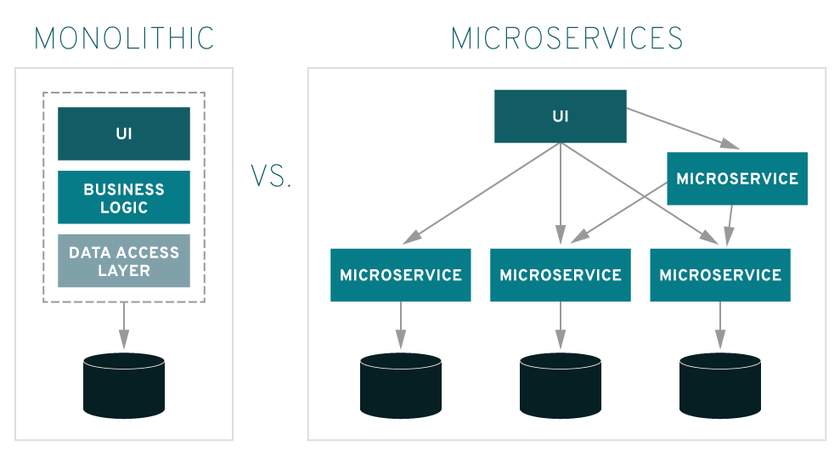
\includegraphics[scale=0.6]{inc/img/Monolithic-vs-microservices.png}
    \caption{Сравнение микросервисной и монолитной архитектуры}
\end{figure}

\section{Технология контейнеризации}
% https://ru.wikipedia.org/wiki/%D0%92%D0%B8%D1%80%D1%82%D1%83%D0%B0%D0%BB%D0%B8%D0%B7%D0%B0%D1%86%D0%B8%D1%8F
По определению виртуализация -- это предоставление набора вычислительных
ресурсов или их логического объединения, абстрагированное от аппаратной
реализации, и обеспечивающее при этом логическую изоляцию друг от друга
вычислительных процессов, выполняемых на одном физическом ресурсе.

% https://habr.com/ru/company/southbridge/blog/530226/
% https://eternalhost.net/blog/razrabotka/docker-kubernetes
Одной из отличительных черт контейнеров от виртуальных машин -- то, что первые
используют возможность не железа, а операционной системы, так называемое
пространство имен. Можно произвести грубое сравнение виртуальных машин и
контейнеров:
% learning docker
\begin{table}[H]
    \centering
    \begin{tabular}{|l|l|}
        \hline
        {\bf Виртуальные машины}                   & {\bf Контейнеры} \\\hline
        Аппаратная виртуализация                   & Виртуализация на уровне ОС \\\hline
        Тяжеловесные                               & Легковесные \\\hline
        Полностью изолированные (более безопасные) & Изолирование на уровне процессов \\\hline
    \end{tabular}
    \caption{Сравнение виртуальных машин и контейнеров}
\end{table}
\begin{figure}[H]
    \centering
    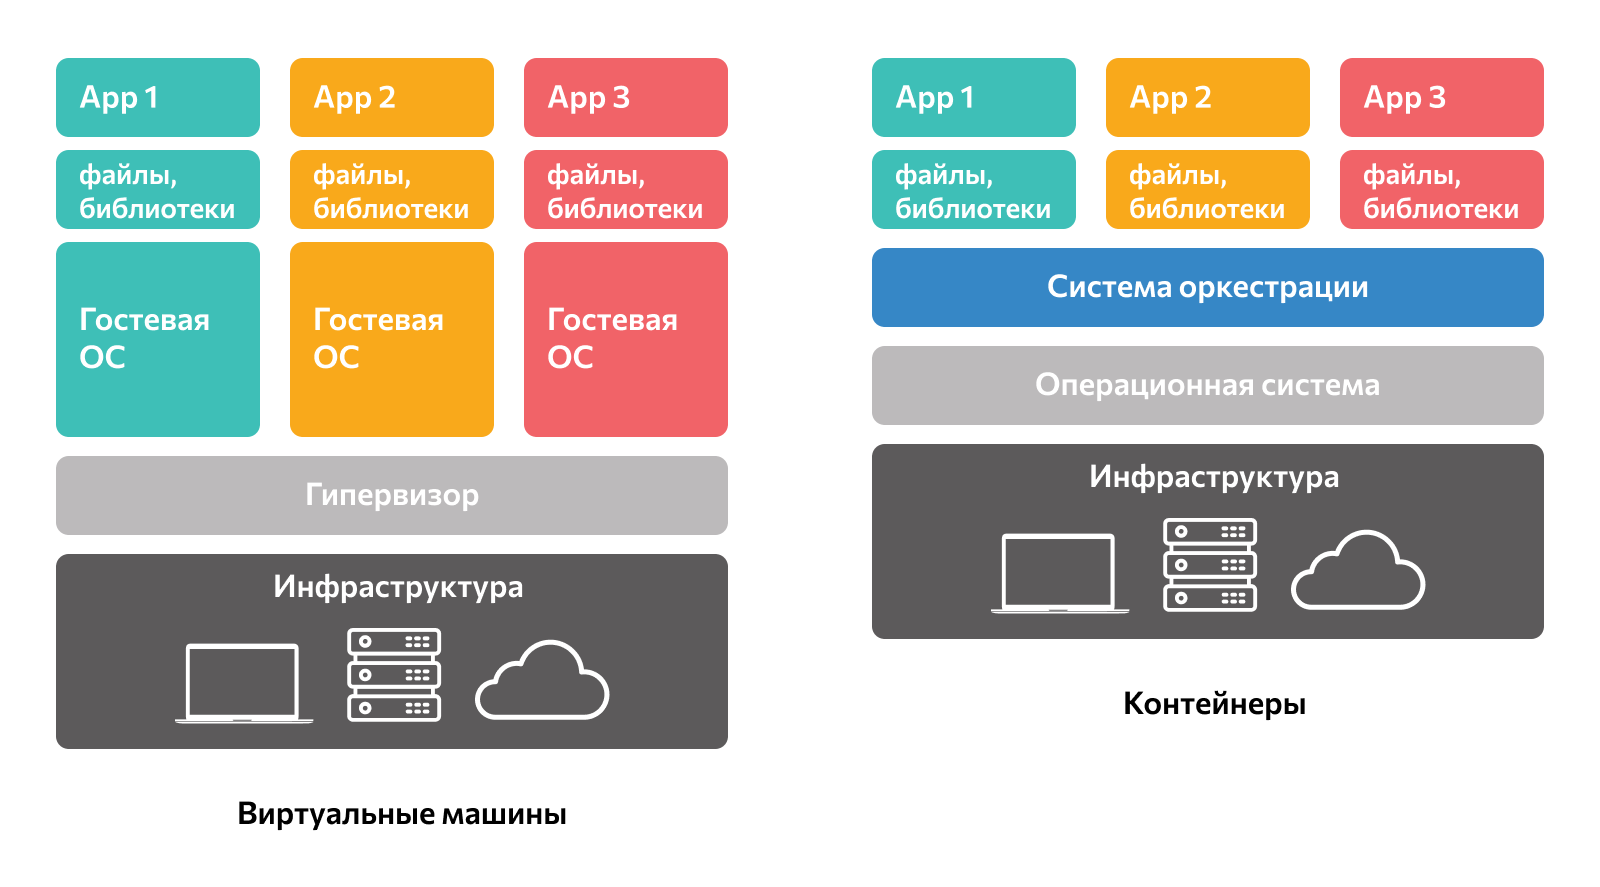
\includegraphics[scale=0.25]{inc/img/cont-vs-virt.png}
    \caption{Сравнение виртуальных машин и контейнеров}
\end{figure}

% https://blog.skillfactory.ru/glossary/kontejnerizacziya/
Технологии контейнеризации решают проблему изолированного запуска приложений и
рабочих сред вне зависимости от системы (должно быть то же ядро) и ПО,
установленных на конкретной машине. Также данная технология позволяет легко
управлять сложными приложениями и средами (упаковывать зависимости, перемещать
решение с системы на систему). 

% TODO: сравнение технологий контейнеризации
\section{Поиск по web-ресурсам}
Для поиска по web-ресурсам безусловно достаточно только возможность совершать
HTTP-запросы (с необходимыми заголовками, сертификатами и т.д.) и читать то, что
сервер возвращает клиенту. Но в целях данной выпускной квалификационной работы
присутствует задача выбрать хорошую архитектуру. Поэтому нужно рассмотреть
фреймворки (или системы), которые позволяют упростить эту самую работу.

% https://pythobyte.com/10-tips-to-avoid-getting-blocked-while-scraping-websites-ncf-bee5b81c/
Также многие сайты стараются скрыть свою информацию от web-ботов. Возможно это
обусловленно тем, что последние злоупотребляют общедоступной информацией либо
вычислительной мощностью, которую сервер выделяет на пользователя. Поэтому, на
таких серверах могут быть настроенны политики запрета доступа к контенту при
слишком частом запросе страницы.

% https://coderlessons.com/tutorials/devops/uchitsia-scrapy/scrapy-kratkoe-rukovodstvo
Свойства которыми должен обладать фреймворк при работе с web-ресурсами:
\begin{itemize}
    \item Быть масштабируемым на большие проекты сканирования;
    \item Асинхронная обработка запросов;
    % TODO: сделать сноску на селекторы
    \item Встроенный механизм работы с селекторами;
    % TODO: сделать сноску на дросселирование
    \item Обладает механизмом автоматического дросселирования;
    \item Генерация результатов в разных структурных текстовых форматах.
\end{itemize}

% сравнение requests, beautiful soup 4, lxml, selenium, scrapy

Фреймворк на python -- scrapy удовлетворяет всем вышеперечисленным свойствам.
Более того для него написанна серверная часть scrapyd, которая позволяет
размещать "пауков" на мощных серверах, с последующим запуском либо по
расписанию, либо по http-запросу.
\begin{figure}[H]
    \centering
    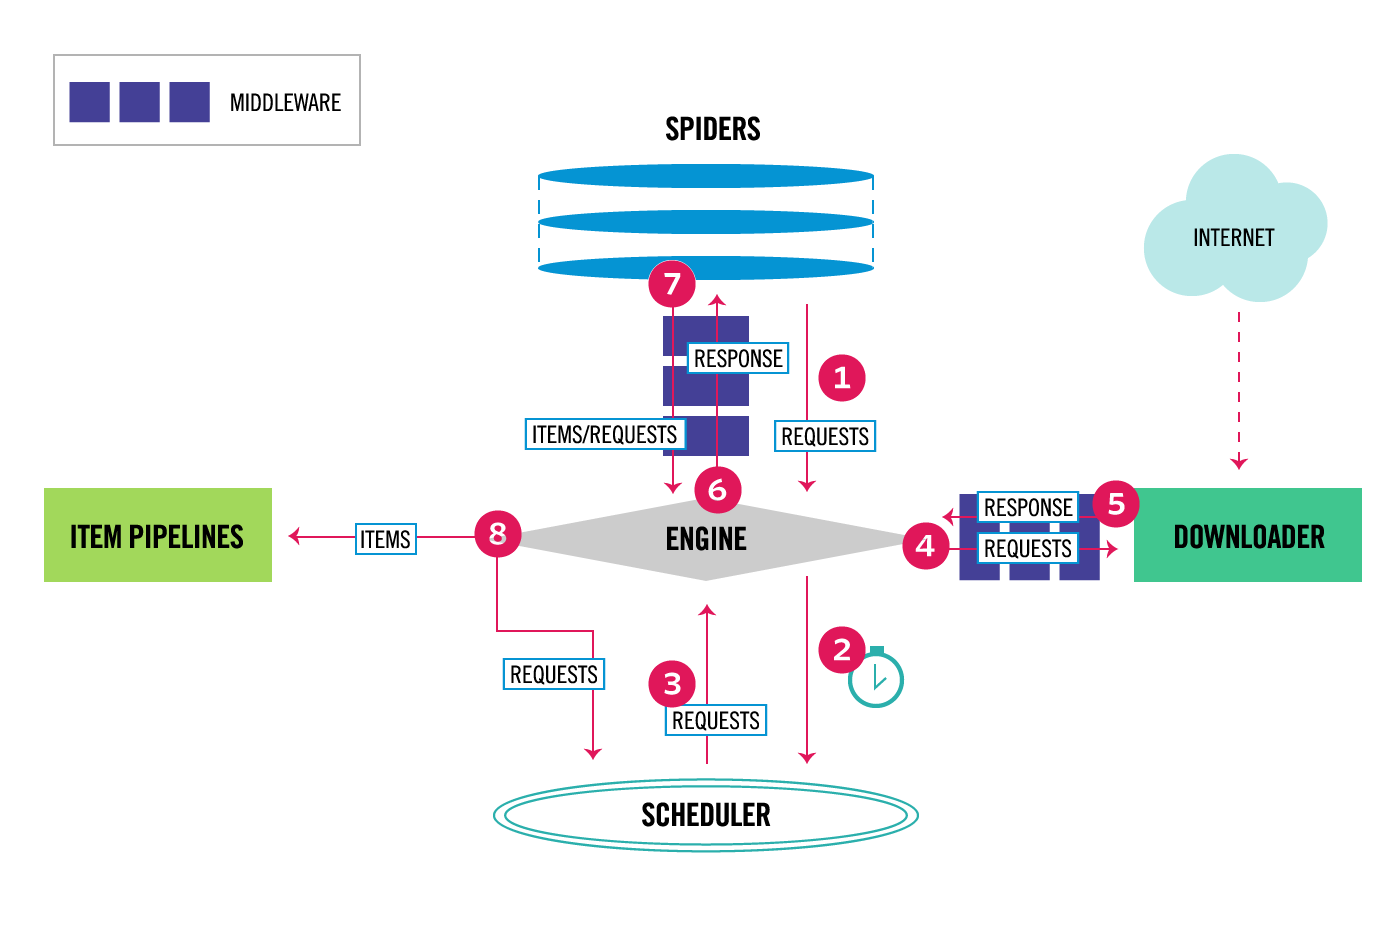
\includegraphics[scale=0.35]{inc/img/scrapy_architecture.png}
    \caption{Архитектура scrapy}
\end{figure}

% TODO: сделать сноску что этот файл обозначает
Также в этом модуле можно настроить много других политик доступа к интернет ресурсам. В такие политики входят:
\begin{itemize}
    \item Чтение файла \verb|robots.txt|;
    \item Лист прокси;
    \item Ротация заголвков и куков.
\end{itemize}

Данная библиотека позволяет полностью посмотреть список настроек, добавить свои,
и написать такую конфигурацию системы, чтобы не добавить свою вычислительную
сеть в черный список целевой структуры.

\section{Серверная часть}
\subsection{Web-сервер}
% https://ru.wikipedia.org/wiki/%D0%92%D0%B5%D0%B1-%D1%81%D0%B5%D1%80%D0%B2%D0%B5%D1%80
Веб-сервер -- сервер, принимающий HTTP-запросы от клиентов, обычно веб-браузеров,
и выдающий им HTTP-ответы, как правило, вместе с HTML-страницей, изображением,
файлом, медиа-потоком или другими данными. Веб-сервером называют как программное
обеспечение, выполняющее функции веб-сервера, так и непосредственно компьютер ,
на котором это программное обеспечение работает.

% https://developer.mozilla.org/ru/docs/Learn/Common_questions/What_is_a_web_server
На самом базовом уровне, когда браузеру нужен файл, размещённый на веб-сервере,
браузер запрашивает его через HTTP-протокол. Когда запрос достигает нужного
веб-сервера ("железо"), сервер HTTP (ПО) принимает запрос, находит запрашиваемый
документ (если нет, то сообщает об ошибке 404) и отправляет обратно, также через
HTTP.
\begin{figure}[H]
    \centering
    
\includegraphics[scale=0.60]{inc/img/web-server.png}
    \caption{Принцип работы web-сервера}
\end{figure}

Хранить ресурсы на выделенном web-сервере удобно по нескольким причинам:
\begin{itemize}
    \item Доступность выше чем у домашнего ПК;
    \item Всегда подключен к Интернету (зависит конечно же от хостера);
    \item Имеет статический IP адрес (с провайдерами обычно приходится договариваться на какую-то сумму, что бы выделили такой же);
    \item Обслуживается сторонней компанией, специализирующейся на предоставлении своего продукта.
\end{itemize}

% http://www.advanserv.ru/lab/stati/webserver/
% https://smoff.ru/howitworks/chto-takoe-nginx
Помимо своих основных функций веб-серверы выполняют и «работу» другого рода:
\begin{itemize}
    \item Запускает другие программные решения на серверных языках программирования;
    \item Защищает информацию от несанкционированного доступа;
    \item Ведет журнал обращений;
    % TODO: сделать сноску на два термина
    \item Обеспечивает аутентификацию и авторизацию;
    \item Обслуживает запросы разных типов: FTP, mailto и др.
\end{itemize}

% https://4db.github.io/2015/02/12/apache-iis-vs-nginx-nodejs/
На сегодняшний день популярными веб серверами являются: Apache, IIS, Nginx,
Node.js. У каждого веб сервера есть своя история, фокус на технологиях,
предпочитаемые ОС и многое другое. Но есть принципиальное различие в процессе
обработки запросов.

Apache, IIS используют обрабатывают каждый запрос в отдельном потоке/процессе -
“process-based”.
\begin{figure}[H]
    \centering
    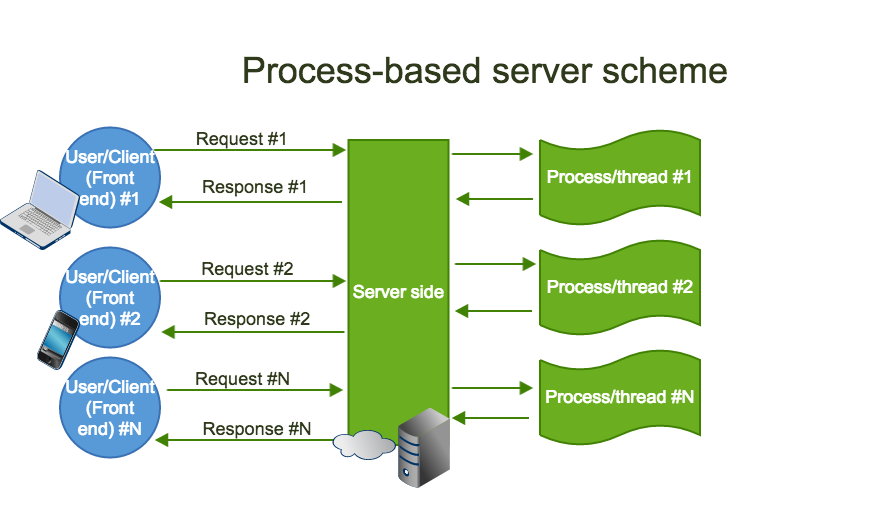
\includegraphics[scale=0.40]{inc/img/process-based-server.png}
    \caption{Схема работы Process-based веб серверов}
\end{figure}

Event-based web serves: Nginx, Node.js. Работают на одном процессе/потоке,
используя все выделенные ресурсы. В единичном процессе/потоке(Singe
process/thread) используются все ресурсы веб сервера, позволяя обрабатывать
запросы максимально быстро, а в случаи задержки(получение данных от клиента,
отправки данных клиенту) работать с другими запросами из очереди(Event Queue)
т.е асинхронно.
\begin{figure}[H]
    \centering
    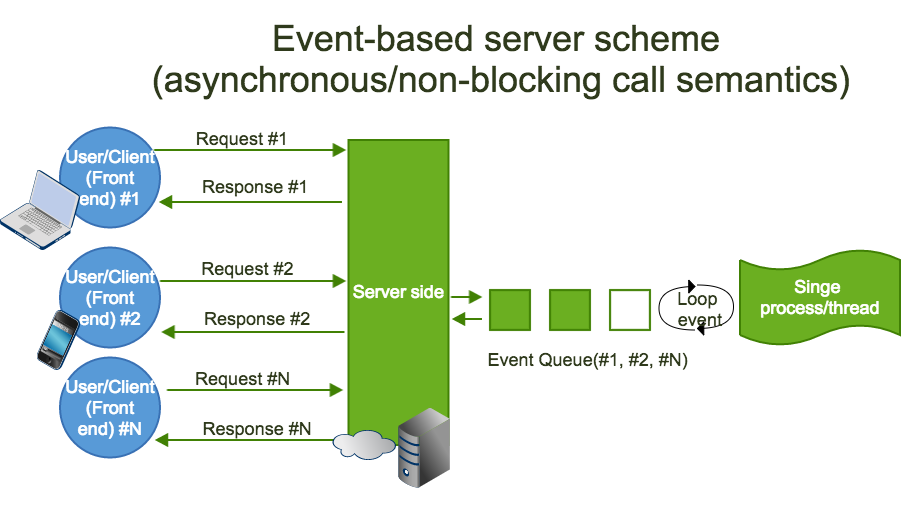
\includegraphics[scale=0.40]{inc/img/event-based-server.png}
    \caption{Схема работы Event-based веб сервера}
\end{figure}

Схема event-based(Node.js, Nginx) показывает большую производительность при
высоких нагрузках. Это связано с тем что не нужно делить ресурсы сервера между
другими потоками/процессами. Также серверные ресурсы всегда используются без
“простоя”.

Учитывая что Nginx обладает дополнительной функциональность (распределитель
нагрузки, вшитые механизмы защиты, прокси сервер), мой выбор пал именно на этот
web-сервер.

\subsection{Web-фреймворк}
% https://web-creator.ru/articles/about_frameworks
Фреймворки -- это программные продукты, которые упрощают создание и поддержку
технически сложных или нагруженных проектов. Фреймворк, как правило, содержит
только базовые программные модули, а все специфичные для проекта компоненты
реализуются разработчиком на их основе. Тем самым достигается не только высокая
скорость разработки, но и большая производительность и надёжность решений.

Веб-фреймворк -- это платформа для создания сайтов и веб-приложений, облегчающее
разработку и объединение разных компонентов большого программного проекта. За
счёт широких возможностей в реализациии бизнес-логики и высокой
производительности эта платформа особенно хорошо подходит для создания сложных
сайтов, бизнес-приложений и веб-сервисов.

Основное отличие библиотеки от фреймворка заключается в том, что последний не
просто дает разработчику нужный функционал, но еще и диктует правила построения
архитектуры приложения, задавая на начальном этапе разработки поведение по
умолчанию, формируя каркас, который нужно будет расширять и изменять согласно
указанным требованиям. Фреймворк также может включать вспомогательные программы,
библиотеки кода, язык сценариев и другое ПО, облегчающее разработку и
объединение разных компонентов большого программного проекта.

Для написания основной логики данной работы был выбран язык Python. Поэтому
рассмотрим основные web-фреймворки из которых стоит выбрать: Django и Flask.

% https://tproger.ru/articles/obzornyj-analiz-python-veb-frejmvorkov/
% TODO: Сделать сноску на MTV
Django диктует достаточно хорошую структуру (сразу подразумевает модульность и
расширяемость, модель MTV). Обширный каталог плагинов обеспечивают широкий выбор
опций для дополнения функциональности. Сразу при установке разработчику доступны
такие инсттрументы как ORM, шаблонизатор, мультиязычность, админ-панель,
автоматическая документация.

Flask позволяет разработчику собственноручно выбрать инструменты для реализации
логики. Обычно разработчики выбирают этот фреймворк для большего контроля над
проектом. По умолчанию Flask предоставляет:
\begin{itemize}
    \item Сервер разработки и отладчик;
    \item Интегрированные инструменты для модульного тестирования;
    \item Возможность отправки REST запросов;
    \item Шаблонизатор Jinja2;
    \item Пакеты-расширения, например flask-login, flask-sqlalchemy, flask-wtf.
\end{itemize}

Так как целевой проект должен получится сравнительно небольшим и по большей
части обучающим, то django слишком упростил бы разработку и не позволил бы
наглядно продемонстрировать используемые инструменты. Поэтому выбор пал на
flask.

\subsection{Коннектор}
% https://www.fullstackpython.com/wsgi-servers.html
% TODO: возможно просто описать стандарт wsgi и что это такое
Так как Nginx выступает в данной архитектуре как обратный прокси, необходим
способ запуска приложения для генерации динамического контента. UWSGI отвечает
за нагрузку приложения Flask с использованием интерфейса WSGI.

WSGI -- спецификация интерфейса. Он указывает какие методы следует использовать
для передачи запросов и ответов между сервером и приложением.

\begin{figure}[H]
    \centering
    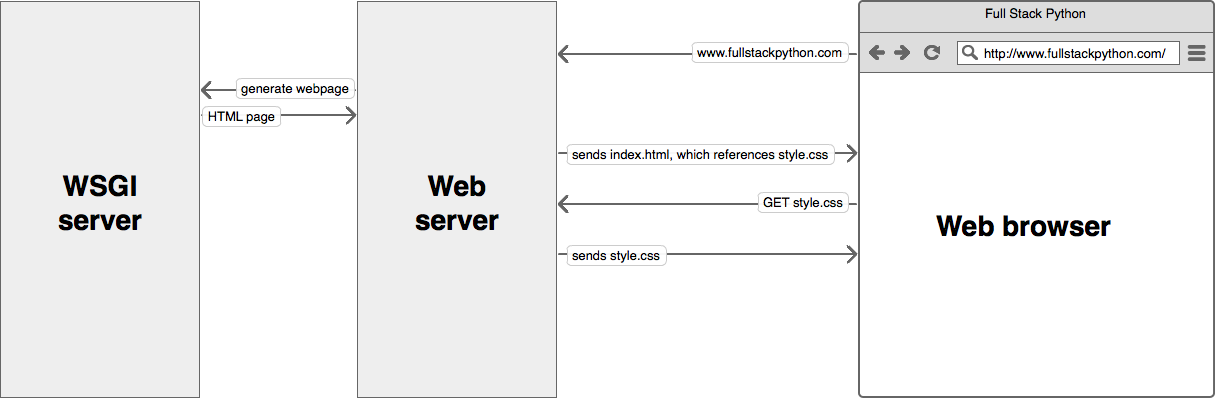
\includegraphics[scale=0.35]{inc/img/web-browser-server-wsgi.png}
    \caption{Роль WSGI сервера в архитектуре приложения}
\end{figure}

\section{Брокер сообщений}
\section{База данных}

